\documentclass[./main.tex]{subfiles}
\begin{document}
\chapter{Architecture}
\section{Espressif's ESP8266}

\begin{figure}[H]
    \centering
    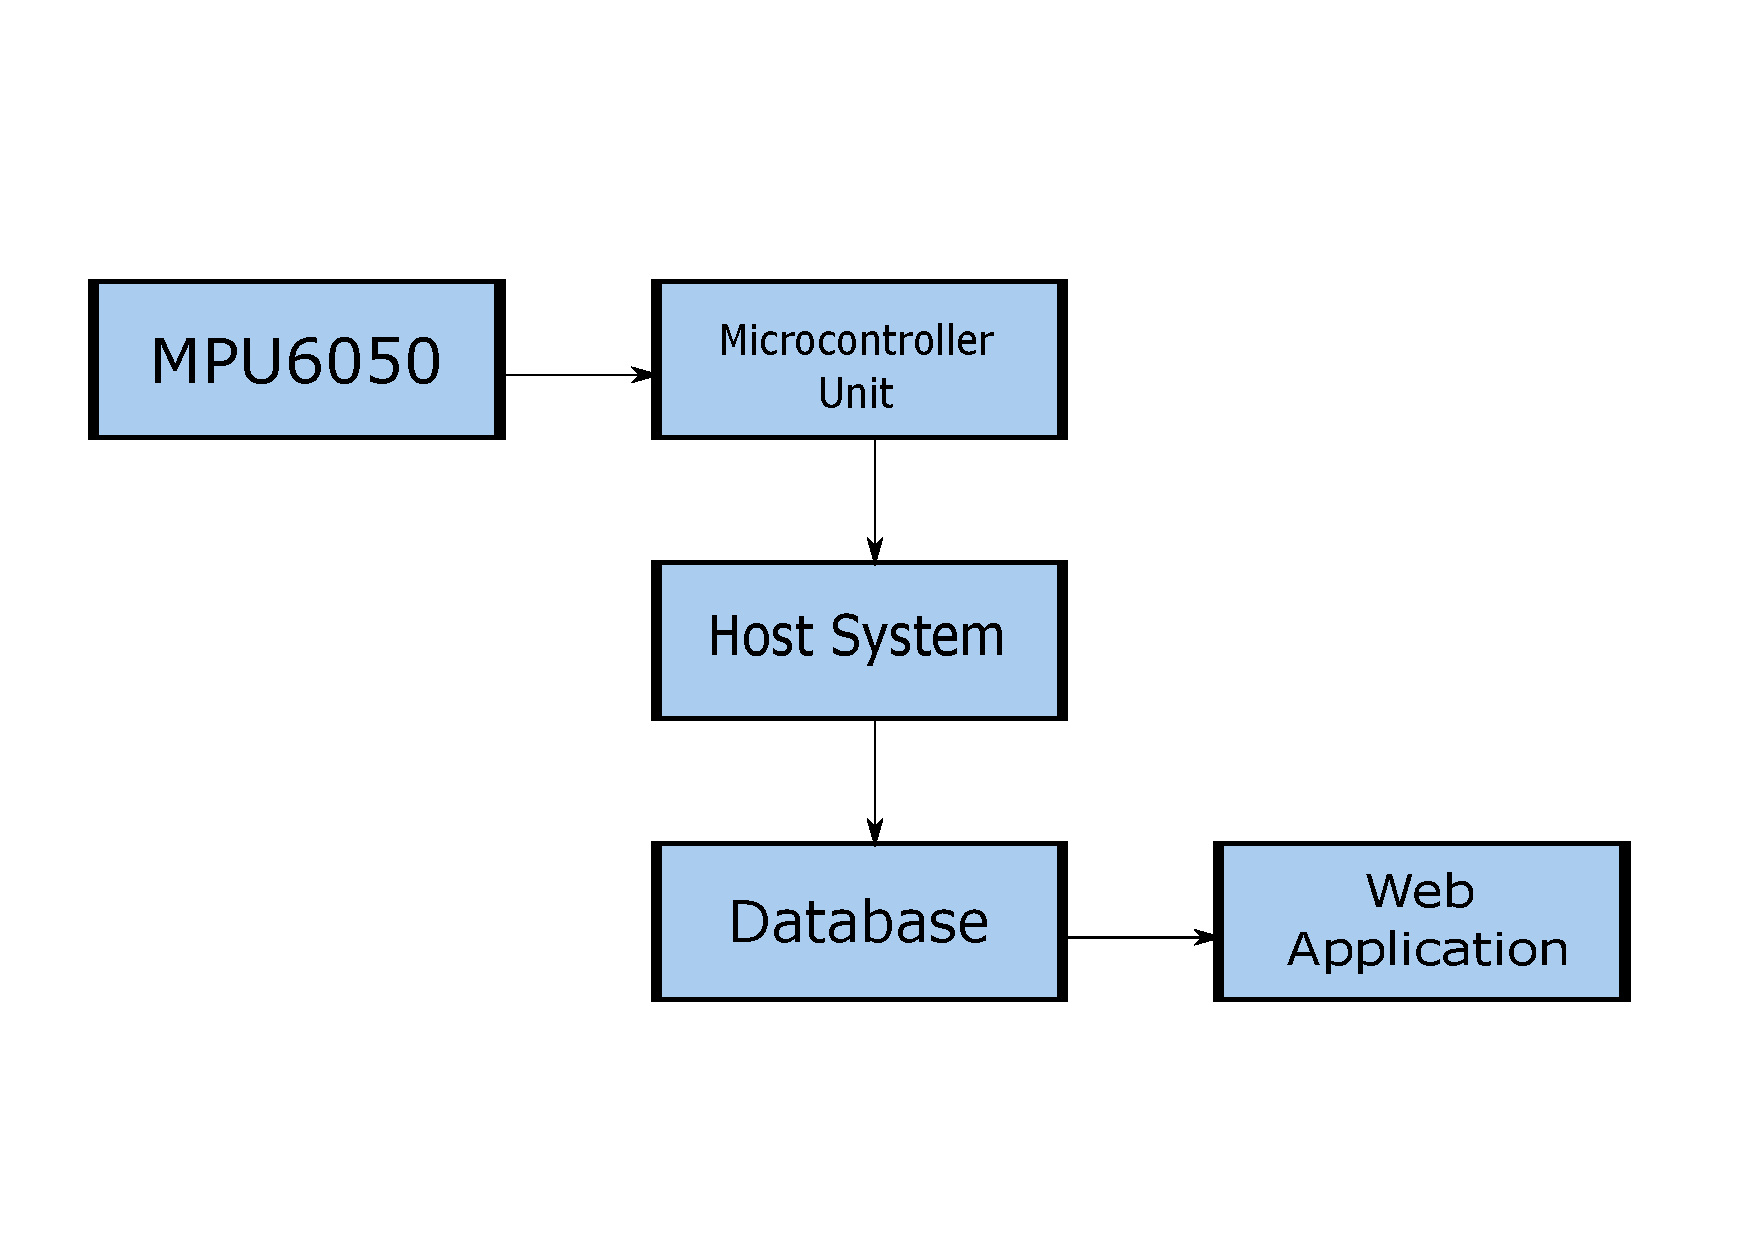
\includegraphics[scale=0.4]{flowchart.pdf}
    \caption{Architecture}
    \label{fig:architecture}
\end{figure}


Espressif’s ESP8266 highly integrated Wi-Fi SoC solution for efficient power
usage, compact design and reliable performance in the Internet of Things
industry. The integrated high-speed cache helps to increase the system
performance and optimize the system memory. \\ Most importantly, ESP8266 also
integrates a 32-bit processor and on-chip SRAM.  It supports UART, SDIO, SPI,
I\textsuperscript{2}C, I\textsuperscript{2}S, IR Remote Control protocols for
communication purposes.  Also, it has 17 GPIO pins which can be assigned to
various functions by programming the appropriate registers \cite{espdata}.

\section{Arduino UNO}
The Arduino Uno is a microcontroller board based on the ATmega328P. It has 14
digital input/output pins (of which 6 can be used as PWM outputs) and 6 analog
inputs. \\ The ATmega328P has 32 KB (with 0.5 KB used for the bootloader). It
also has 2 KB of SRAM and 1 KB of EEPROM. The ATmega328 also supports
I\textsuperscript{2}C (TWI) and SPI communication \cite{arddata}.

\section{MPU6050 Gyro-Accelerometer}
The MPU6050 contains a MEMS (Micro-electromechanical System) 3-axis gyroscope
and a 3-axis accelerometer on the same silicon die together with an on-board
Digital Motion Processor. \\ The MPU-6050 has three 16-bit analog-to-digital
converters (ADCs) each for digitizing the gyroscope outputs and the
accelerometer outputs \cite{mpudata}. For our application, the connections
between MPU6050 Gyro-Accelerometer and the ESP8266 Microcontroller are as
follows:

\begin{table}[H]
    \centering
    \begin{tabular}{|c|c|}
    \hline
    MPU6050 Gyro-Accelerometer & ESP8266 Microcontroller \\
    \hline
    VCC & VCC (3.3V) \\
    GND & GND \\
    SCL & D1 \\
    SDA & D2 \\
    \hline
    \end{tabular}
    \caption{Pin connections between the sensor and the microcontroller}
    \label{tab:pin}
\end{table}

\end{document}
